\documentclass{amsart}

\usepackage[notref,notcite]{showkeys}
\usepackage[style=authoryear,ibidtracker=false,uniquename=false,giveninits=true,terseinits=true,maxbibnames=5,backend=biber]{biblatex}
\usepackage{float}
\usepackage{graphicx}
\usepackage{todonotes}
\usepackage{subcaption}
\usepackage{amsmath}
\usepackage{amsthm}
\usepackage{amssymb}
\usepackage[foot]{amsaddr}
\usepackage[misc]{ifsym}
\usepackage{enumitem}

\setlist{leftmargin = 0pt, labelindent = 0pt}

\renewbibmacro{in:}{}
\addbibresource{rnni_polynomial.bib}

\newtheorem{lemma}{Lemma}
\newtheorem{theorem}{Theorem}

\newcommand{\rnni}{\mathrm{RNNI}}
\newcommand{\findpath}{\textsc{FindPath}}
\newcommand{\mrca}{\mathrm{mrca}}
\newcommand{\rank}{\mathrm{rank}}
\newcommand{\nni}{\mathrm{NNI}}
\newcommand{\fp}{\mathrm{FP}}
\renewcommand{\O}{\mathcal O}

\renewcommand{\thesubfigure}{\Alph{subfigure}}

\graphicspath{{figures/}}


\title[Computing $\rnni$ distance]{Efficient algorithm for computing nearest neighbour interchange distance between ranked phylogenetic trees}
\date{\today}
\author{Lena Collienne\textsuperscript{1}}
\email{lena.collienne@postgrad.otago.ac.nz}
\address{\textsuperscript{1}Department of Computer Science, University of Otago, New Zealand}
\author{Alex Gavryushkin\textsuperscript{1, \Letter}}
\email{\textsuperscript{\Letter}alex@biods.org}


\begin{document}

\begin{abstract}
We present a quadratic algorithm to compute shortest paths, and hence the distance, between ranked phylogenetic trees under the ranked nearest neighbour interchange operation.
\end{abstract}


\maketitle

Things to introduce:

\begin{itemize}
\item Trees with the notion of an interval in a tree (if we want intervals), clusters, clusters induced by nodes, subtrees induced by clusters, list representation of trees.
\item $(T)_k$: node of rank k, $(C)_T$: mrca of cluster $C$ in $T$
\item $\findpath$, including its time complexity.
\item Note that $\findpath$ is deterministic, that is, an interval and a move on the interval are uniquely determined (this is necessary to concentrate on the $v, w$ nodes in the proof of main theorem).
\end{itemize}

\begin{theorem}
The time complexity of computing the $\rnni$ distance between trees on $n$ leaves is $\O(n^2)$.
\end{theorem}

\proof
We prove this theorem by showing that for every pair of trees $T$ and $R$, the path computed by the $\findpath$ algorithm is a shortest $\rnni$ path.
We denote this path by $\fp(T, R)$ and its length by $|\fp(T, R)|$.

Assume to the contrary that $T$ and $R$ are two trees with a minimum possible distance $d(T, R)$ such that $d(T,R) \neq |\fp(T,R)|$, that is, $d(T,R) < |\fp(T,R)|$.
Let $T'$ be the first tree on a shortest $\rnni$ path from $T$ to $R$.
Then $d(T',R) = d(T, R) - 1$ and the distance between $T'$ and $R$ is strictly smaller than that between $T$ and $R$.
Hence $d(T', R) = |\fp(T',R)| < |\fp(T,R)| - 1$.
We finish the proof by showing that no trees satisfy this inequality.

Specifically, we will show that for all trees $T$, $R$, and $T'$ such that $T'$ is one $\rnni$ move away from $T$,
\begin{equation}
	|\fp(T',R)| \geq |\fp(T,R)| - 1
 	\label{eqn:iff_inequality}
\end{equation}

We will use Figure~\ref{fig:proof_idea} to demonstrate our argument.

\begin{figure}[!hbt]
\centering
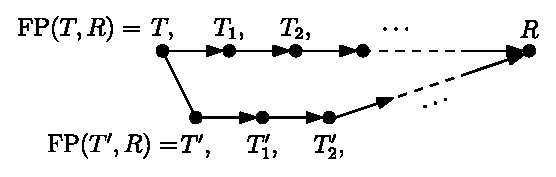
\includegraphics[width=0.6\textwidth]{proof_idea_ag}
\vspace{12pt}
\caption{Trees $T$, $T'$, and $R$ as in inequality~(\ref{eqn:iff_inequality}).
Paths $p = \fp(T,R) = [T,T_1,T_2, \ldots, R]$ and $p' = \fp(T',R) = [T',T'_1,T'_2, \ldots, R]$ are indicated by arrows.}
\label{fig:proof_idea}
\end{figure}

Assume to the contrary that $T$ and $R$ are trees for which there exists $T'$ violating inequality~(\ref{eqn:iff_inequality}).
Out of all such pairs $T, R$ choose one with the minimal $|\fp(T, R)|$.
Denote $\fp(T,R) = [T, T_1, T_2, \ldots, R]$ by $p$ and $\fp(T', R) = [T', T_1', T_2', \ldots, R]$ by $p'$, and let $[(T)_t, (T)_{t+1}]$ be the interval in $T$ on which the $\rnni$ move connecting $T$ and $T'$ is performed.
Let $C_k$ be the cluster of $R$ such that the node $(C_k)_T$ is moved down by the first move on $p$.
If the rank of $(C_k)_T$ is not in $\{t, t+1\}$ then $(C_k)_T$ and $(C_k)_{T'}$ induce the same cluster, so $\findpath$ would make the same rearrangement in both trees $T$ and $T'$ in the first move along $p$ and $p'$ resulting in trees $T_1$ and $T_1'$ which are $\rnni$ neighbours, as in Figure~\ref{fig:proof_idea}.
In this case, paths $\fp(T_1, R)$ and $\fp(T_1', R)$ violate inequality~(\ref{eqn:iff_inequality}) but $\fp(T_1, R)$ is strictly shorter than $\fp(T, R)$, contradicting our minimality assumption.
Hence, the first move on $p$ has to involve an interval incident to at least one of the nodes $(T)_t$, $(T)_{t+1}$.

We will distinguish two cases depending on whether $T$ and $T'$ are connected by an $\nni$ or a rank move.
For each of these we will further distinguish all possible moves between $T$ and $T_1$.

\textbf{Case 1.} $T$ and $T'$ are connected by an $\nni$ move, so $((T)_t,(T)_{t+1})$ is an edge in $T$ -- see Figure~\ref{fig:thm_fp_nni1}.
Denote the clusters induced by the children of $(T)_t$ by $A$ and $B$ and the cluster induced by the child of $(T)_{t+1}$ that is not $(T)_t$ by $C$, and assume that the $\nni$ move between $T$ and $T'$ exchanges the subtrees induced by clusters $B$ and $C$.

\begin{figure}[!hbt]
\centering
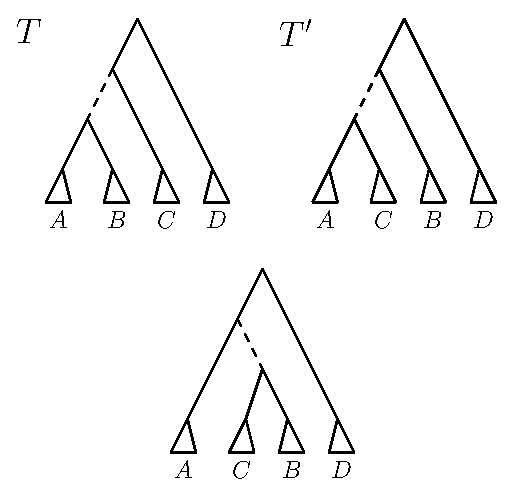
\includegraphics[width=0.4\textwidth]{thm_fp_nni1}
\vspace{12pt}
\caption{$\nni$ move between $T$ and $T'$ on the dashed edge $((T)_t,(T)_{t+1})$ and the third $\rnni$ neighbour resulting from a move on that edge.}
\label{fig:thm_fp_nni1}
\end{figure}

We now consider all possible moves $\findpath$ can perform to go from $T$ to $T_1$ that involve a node of rank $t$ or $t+1$, that is, we will consider three intervals in total.

\begin{enumerate}[label = 1.{\arabic*}]
\item An $\rnni$ move on interval $[(T)_t, (T)_{t+1}]$.
Note that this move has to be the $\nni$ move that is different from the $\nni$ move connecting $T$ and $T'$.

In this case, the cluster $B \cup C$ is built in $T_1$, as depicted in the bottom of Figure~\ref{fig:thm_fp_nni1}.
It follows that the cluster $C_k$ that is considered first by $\findpath$ must contain taxa from both $B$ and $C$.
But then $\findpath$ applied to $T'$ and $R$ has to decrease the rank of $(C_k)_{T'}$ in its first step implying that $T'_1 = T_1$.
Hence $|\fp(T',R)| = |\fp(T,R)|$, which contradicts our assumption that $|\fp(T',R)| < |\fp(T,R)| - 1$.

\item An $\nni$ move on interval $[(T)_{t+1}, (T)_{t+2}]$.
This case implies that $((T)_{t+1},(T)_{t+2}))$ is an edge in $T$.

We use the same notations for clusters $A$, $B$, and $C$ as above and additionally denote the cluster induced by the child of $(T)_{t+2}$ that is not $(T)_{t+1}$ by $D$ --
\todo{Why does the same tree appear in the second row, second column twice?}
see Figure~\ref{fig:thm_fp_nni2a}.
Note that the position of the tree root is irrelevant for our argument, so we have placed the root to simplify the figures.

\begin{figure}[H]
	\begin{subfigure}[b]{.45\textwidth}
		\centering
		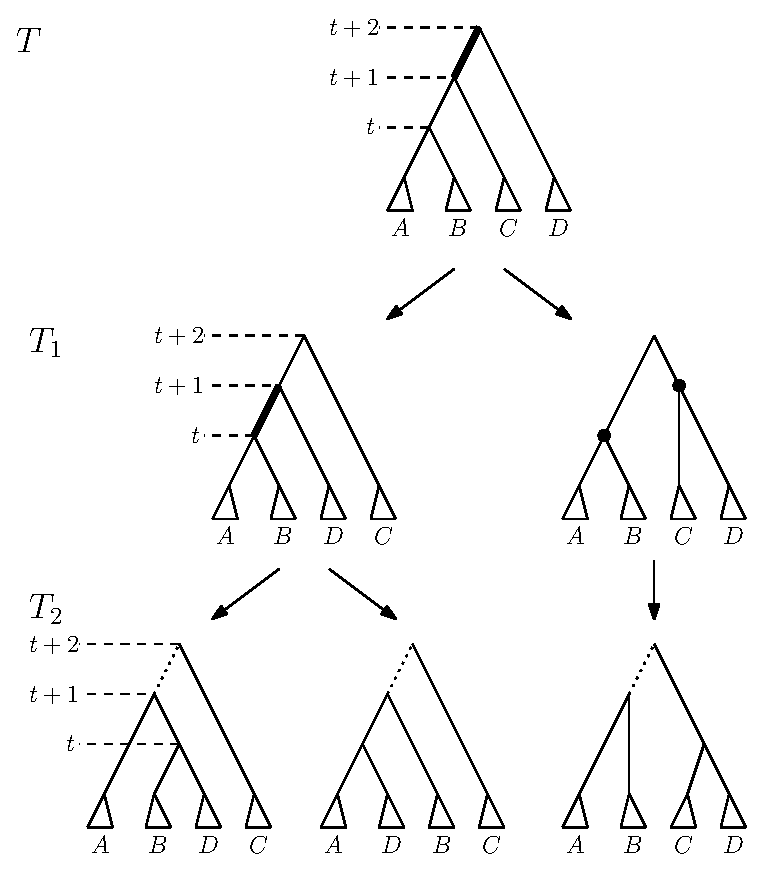
\includegraphics[width=0.9\linewidth]{thm_fp_nni2a.eps}
		\vspace{12pt}
		\caption{path $p$ following $T$}
		\label{fig:thm_fp_nni2a}
	\end{subfigure}
	\begin{subfigure}[b]{.45\textwidth}
		\centering
		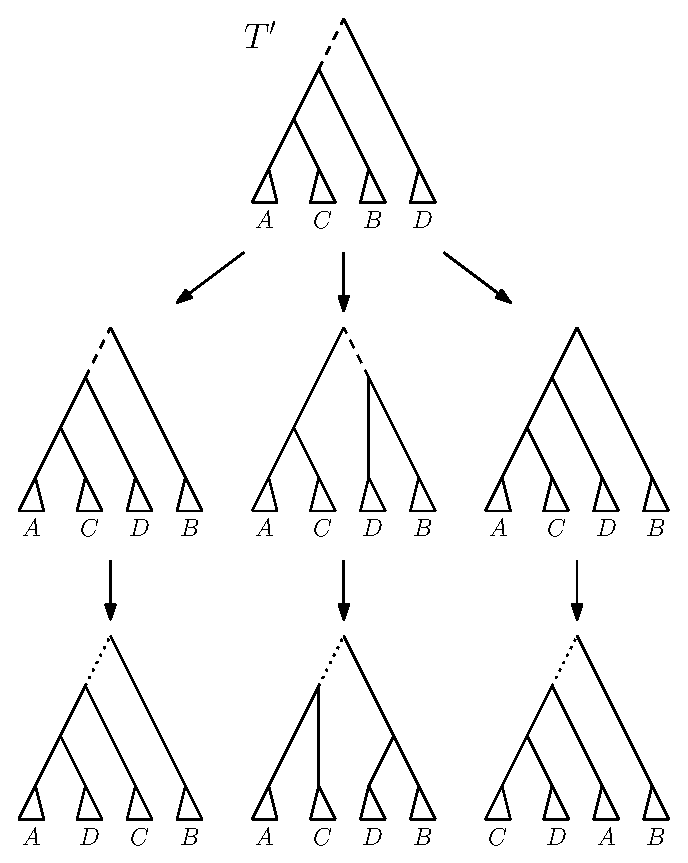
\includegraphics[width=0.9\linewidth]{thm_fp_nni2b.eps}
		\vspace{12pt}
		\caption{path $p'$ following $T'$}
		\label{fig:thm_fp_nni2b}
	\end{subfigure}
	\caption{Comparison of $p$ and $p'$ if there is an $\nni$ move on the edge $((T)_{t+2},T_{t+1})$ in $T$.
	The bottom row displays all possibilities for $T_2$ and $T'_2$, depending on the position cluster $C_k$ that is considered by $\findpath$:
	${C_k \subseteq A \cup D}$ is on the left, ${C_k \subseteq B \cup D}$ is in the middle, ${C_k \subseteq C \cup D}$ is on the right.}
\end{figure}

\todo{Not sure if we need this paragraph.}
We will now consider each $\nni$ move that could possibly happen on $\findpath$ on $T$ resulting in $T_1$, separately.
If $T_1$ is the tree at the top left of Figure~\ref{fig:thm_fp_nni2a}, resulting from $T$ by exchanging the subtrees induced by $C$ and $D$, the cluster $C_k$, the most recent common ancestor of which is moved down by $\findpath$, contains elements of $D$ and of $A \cup B$.
In the following we distinguish three cases, depending on whether $C_k$ contains, besides taxa of $D$, just taxa of $A$ or $B$, or both.
\todo{This presumes that $k > 1$.}
We denote the cluster $(R)_{k-1}$ by $C_{k-1}$.

\begin{enumerate}[label = \theenumi.\arabic*]
    \item If $C_k$ contains elements of all three clusters $A, B$ and $D$, then $C_{k-1} = A \cup B$ as the two clusters of $R$ that join to $C_k$ in $R$ must already be present in $T$.
	\todo{LC: Is this clear?}
    As this $C_{k-1} = A \cup B$ is no cluster of $T'$, the move $\findpath$ makes on $T'$ decreases the rank of $(C_{k-1})_{T'}$ before $C_k$ is considered by the algorithm.
    This $\rnni$ move on $T'$ decreases the rank of $(C_{k-1})_{T'}$ by building the cluster $A \cup B$, such that $T'_1 = T$.
	This however contradicts $|\fp(T',R)| < |\fp(T,R)| - 1$.

    \item If $C_k \subseteq A \cup D$, the move on $T_1$ decreases the rank of $(C_k)_{T_1}$ by exchanging $B$ and $D$, resulting in the tree  $T_2$ as depicted in the bottom left of Figure~\ref{fig:thm_fp_nni2a}.
	As $C_k \subseteq A \cup D$, we can follow that from $T'$ to $T'_1$ to $T'_2$ the rank of $(C_k)_{T'}$ decreases by two by exchanging the subtree induced by $D$ with the ones induced by $B$ and $C$ as depicted on the left of Figure~\ref{fig:thm_fp_nni2b}.
	It follows that $T_2$ and $T'_2$ only differ by one interval (dotted edges in the trees at the bottom left of Figures~\ref{fig:thm_fp_nni2a} and~\ref{fig:thm_fp_nni2b}), and hence are $\rnni$ neighbours.
	This together with the fact that $|\fp(T_2,R)| = |\fp(T,R)|-2$ and  $|\fp(T'_2,R)| = |\fp(T',R)|-2$ contradicts the assumption that $\fp(T,R)$ has minimum length among all $\findpath$ paths between pairs of trees violating inequality~(\ref{eqn:iff_inequality}).

	\item
	The case $C_k \subseteq B \cup D$ is analogous to the previous one.
    The two $\rnni$ moves following $T$ and $T'$ on $p$ and $p'$, respectively, end up in trees $T_2$ and $T'_2$ as depicted in the trees in the middle at the bottom of Figures~\ref{fig:thm_fp_nni2a} and \ref{fig:thm_fp_nni2b} that are $\rnni$ neighbours.
    As in the previous case, $T_2, T'_2$ and $R$ violate inequality~(\ref{eqn:iff_inequality}) and $|\fp(T_2,R)| < |\fp(T,R)|$, which contradicts our assumptions on $T$ and $R$.
\end{enumerate}

The second $\nni$ move possible on $((T)_{t+2},(T)_{t+1})$ builds the cluster $C \cup D$ in $T_1$ as illustrated on the right of Figure~\ref{fig:thm_fp_nni2a}.
Hence it is $C_k \subseteq C \cup D$.
If $(C_k)_T$ does not move further down on $p$, $C_{k-1} = A \cup B$ is a cluster in $R$.
As this cluster is not present in $T'$, the $\rnni$ move that $\findpath$ does on this tree builds the cluster $A \cup B$, resulting in $T'_1 = T$, which contradicts $|\fp(T',R)| < |\fp(T,R)| - 1$.
If on the other side the rank of $(C_k)_{T_1}$ decreases further on $p$, the rank of $(C_k)_{T'}$ decreases by at least two on $p'$ as well.
As $C_k \subseteq C \cup D$, these two moves on $p'$ are $\nni$ moves exchanging the subtree induced by $D$ with the ones induced by $B$ and $A$.
These moves are shown on the right of Figure~\ref{fig:thm_fp_nni2b}.
We end up in the same contradiction as in the previous case as the trees $T_2, T'_2$ and $R$ violate inequality~(\ref{eqn:iff_inequality}) and $|\fp(T_2,R)| < |\fp(T,R)|$.

\item A rank move on interval $[(T)_{t+1},(T)_{t+2}]$

Notice that this is only possible if this is a rank interval.
If this rank move is followed by a further rank move, decreasing the rank of $(C_k)_{T_1}$ further, there are two rank moves decreasing the rank of $(C_k)_{T'}$ on $p'$ as well.
The trees $T_2$ and $T'_2$ after these two moves on $p$ and $p'$ coincide in all but one interval.
As previously, this contradicts the assumption that $T$ and $R$ are the closest trees that violate inequality~(\ref{eqn:iff_inequality}).
If on the other side there is no such rank move on $T_1$, it is $C_{k-1} = A \cup B$.
It follows $T'_1 = T$ as this tree results from building $C_{k-1}$ in $T'$, which happens right before $C_k$ is considered by $\findpath$ on $p'$.
This contradicts $|\fp(T',R)| < |\fp(T,R)| - 1$.
\todo{LC: Add a figure for this case?}

\item $\rnni$ move on interval $[(T)_{t},(T)_{t-1}]$

In this case it is $C_k \subseteq A \cup B$.
Hence the move decreasing the rank of $(C_k)_{T'}$ is an $\nni$ move exchanging $B$ and $C$.
This results in $T'_1 = T$, which contradicts $|\fp(T',R)| < |\fp(T,R)| - 1$.
\end{enumerate}

\textbf{Case 2.} Let us now assume that there is a rank move between $T$ and $T'$ where nodes $(T)_{t+1}$ and $(T)_t$ inducing clusters $A$ and $B$ swap ranks as depicted at the top of Figure~\ref{fig:thm_fp_rank1}.
We denote the clusters joining to clusters $A$ and $B$ in $T$ by $A_1,A_2$ and $B_1,B_2$, respectively.
We will again consider the different moves from $T$ to $T_1$ that are possible on intervals incident to $(T)_{t+1}$ or $(T)_{t}$ and show that each of these cases ends in a contradiction, proving that $T,T'$ and $R$ cannot violate inequality~(\ref{eqn:iff_inequality}).

\begin{figure}[!hbt]
\centering
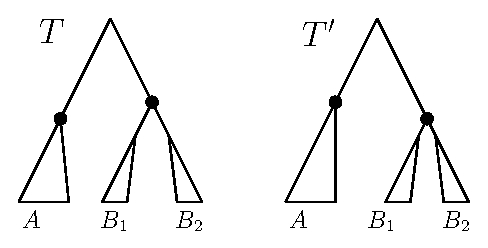
\includegraphics[width=0.4\textwidth]{thm_fp_rank1}
\vspace{12pt}
\caption{Rank move between $T$ and $T'$ on the interval given by the highlighted nodes, and an $\nni$ move on $T$ if the edge $((T)_{t+2},(T)_{t+1})$ has length one.}
\label{fig:thm_fp_rank1}
\end{figure}

\begin{enumerate}[label = 2.\arabic*]
\item Rank move on $[(T)_{t+1},(T)_t]$

This move on $T$ results in $T_1 = T'$.
It follows $|\fp(T',R)| = |\fp(T,R)| - 1$, which contradicts $|\fp(T',R)| < |\fp(T,R)| - 1$.

\item $\nni$ move on edge $((T)_{t+2},(T)_{t})$

Notice that this is only possible if this interval is an edge.
We first assume that $(T)_{t+2}$ is parent of $(T)_t$ and consider the other case later.

\begin{enumerate}
    \item $(T)_{t+2}$ is parent of $(T)_t$

    Then the $\nni$ move on $T$ builds a cluster $A \cup B_i$ for $i \in \{1,2\}$ in $T_1$, which implies $C_k \subseteq A \cup B_i$.
    We assume without loss of generality that this cluster is $A \cup B_1$, as it is depicted on the left of Figure~\ref{fig:thm_fp_rank1}.
    If there is no move decreasing the rank of $(C_k)_{T_1}$ further, it follows $C_{k-1} = A$ and in particular $(C_k)_T = (C_k)_R$.
    Therefore, the first move on $T'$ decreases $(C_{k-1})_{T'}$, which results in $T'_1 = T$, contradicting $|\fp(T',R)| < |\fp(T,R)| - 1$.
    Let us now assume the second option that $(C_k)_{T_1}$ is moved further down on $p$.
    Due to symmetry we can assume that $C_k \subseteq A_1 \cup B_1$, which means that from $T_1$ to $T_2$ the subtrees induced by $A_2$ and $B_1$ exchange by an $\nni$ move, as depicted on the left of Figure~\ref{fig:thm_fp_rank1}.
    From $C_k \subseteq A_1 \cup B_1$ we can infer that the two moves on $p'$ following $T'$ are two $\nni$ moves that result in a tree $T'_2$ that is $\rnni$ neighbour of $T_2$, as depicted on the bottom of Figure~\ref{fig:thm_fp_rank1}.
    This however is a contradiction to the minimality assumption on $|\fp(T,R)|$.

    \item $(T)_{t+2}$ is not parent of $(T)_t$

    In this case the $\nni$ move builds a new cluster $C \cup B_i$ for an $i \in \{1,2\}$ where $C$ is the cluster induced by the child of $(T)_{t+2}$ that does not induce $B$, as depicted in the top left of Figure~\ref{fig:thm_fp_rank2}.
    We can assume without loss of generality that $C_k \subseteq C \cup B_1$.
    If there was no rank move on $T_1$ decreasing the rank of $(C_k)_{T_1}$ further, it is $C_{k-1} = A$, which implies that $A$ is induced by internal node of rank $t$ in both $T$ and $R$.
    Then the rank of $(A)_{T'}$ decreases by a rank move on $p'$ as $C_{k-1} = A$ moves to its final position on $\findpath$ before $C_k$ is considered, which results in $T'_1 = T$.
    This however contradicts $|\fp(T',R)| < |\fp(T,R)| - 1$.

    The case that the rank of $(C_k)_{T_1}$ decreases further on $p$ is depicted on the left of Figure~\ref{fig:thm_fp_rank2}.
    As it is $C_k \subseteq C \cup B_1$, the rank of $(C_k)_{T'}$ decreases by a rank swap of $(C \cup B)_{T'}$ and $(A)_{T'}$ on $T'$ before the subtrees inducing $B_2$ and $C$ exchange by an $\nni$ move, as it is depicted on the right in the same figure.
    One can easily see that $T_2$ and $T'_2$ are $\rnni$ neighbours.
    Again, this is a contradiction to the minimality assumption of $|\fp(T,R)|$.
\end{enumerate}

\begin{figure}[!hbt]
	\centering
	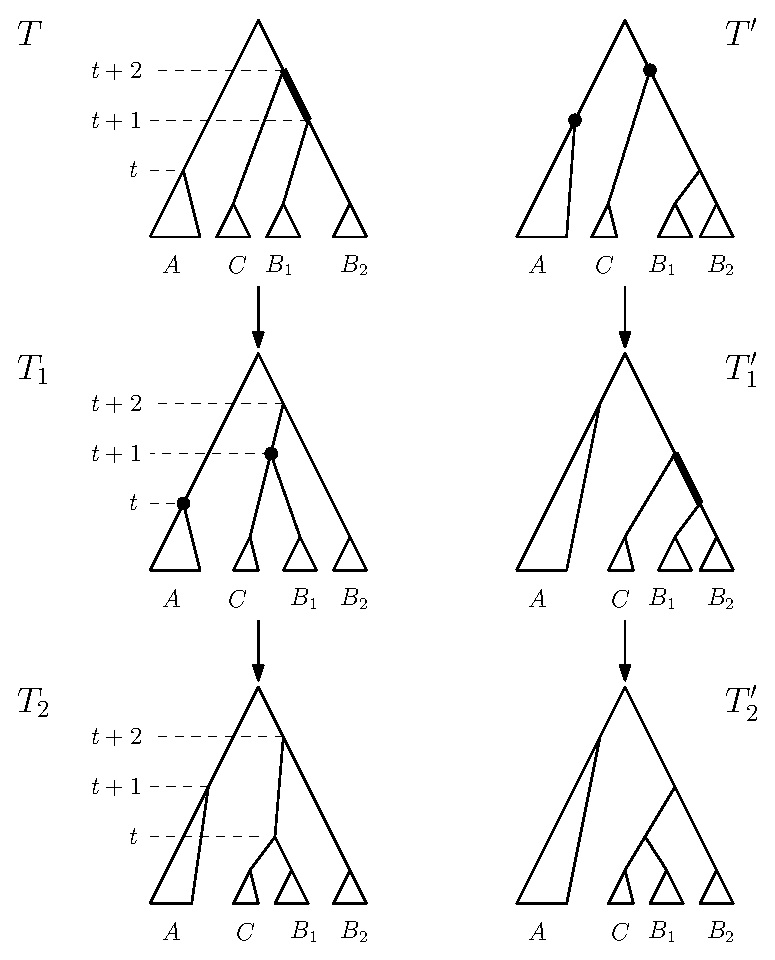
\includegraphics[width=0.4\textwidth]{thm_fp_rank2}
	\vspace{12pt}
	\caption{Comparison of $p$ (left) and $p'$ (right) if there is a rank move between $T$ and $T'$ and an $\nni$ move on the edge below the corresponding rank interval follows on $p$.}
	\label{fig:thm_fp_rank2}
\end{figure}

\item Rank move on interval $[(T)_{t+2}, (T)_{t+1}]$

If no rank move increasing the rank of $(T_1)_{t}$ follows this move, $C_k$ reaches it's final position in the tree $T_1$.
Then it is $C_k = A$, induced by $(T)_t$ in $T$.
It follows that the move on $T$ done by $\findpath$ results in $T$, as $(C_{k-1})_{T'}$ moves down before $C_k$ is considered on $p'$.
This however contradicts $|\fp(T',R)| < |\fp(T,R)| - 1$.
If on the other side the rank swap on $T$ is directly followed by the rank swap of $(T_1)_t$ and $(T_1)_{t+1}$, such rank swaps happen on $p'$ as well and $T_2$ and $T'_2$ are $\rnni$ neighbours.
This is again a contradiction to our choice of $T$ and $R$.

\item $\rnni$ moves on interval $[(T)_{t-1},(T)_t]$

It follows $C_k \subseteq A$.
For decreasing the rank of $(C_k)_{T'}$, the move on $T'$ must be a rank swap resulting in $T$, which contradicts  $|\fp(T',R)| < |\fp(T,R)| - 1$.
\end{enumerate}

We can conclude that in any of the above cases we end up in a contradiction, proving that a tree $T'$ that is $\rnni$ neighbour of $T$ with $|\fp(T',R)| < |\fp(T,R)| - 1$ does not exist.
Therefore we can follow that $|\fp(T',R)| \geq |\fp(T,R)| -1$ for all $\rnni$ neighbours $T'$ of $T$.
\endproof

\end{document}
